% !TEX program = xelatex
%% Requires compilation with XeLaTeX or LuaLaTeX
\documentclass[10pt,xcolor={table,dvipsnames},t]{beamer}
\usepackage{biblatex}
\usepackage{caption}
\setbeamertemplate{caption}[numbered]
\addbibresource{reference.bib}
\usepackage{hyperref}
\hypersetup{ 
pdfpagemode=FullScreen,  
colorlinks=true,linkcolor=blue}
\usepackage{enumerate}

\usepackage{listings}
\usepackage{xcolor}

\definecolor{codegreen}{rgb}{0,0.6,0}
\definecolor{codegray}{rgb}{0.5,0.5,0.5}
\definecolor{codepurple}{rgb}{0.58,0,0.82}
\definecolor{backcolour}{rgb}{0.95,0.95,0.92}

\lstdefinestyle{mystyle}{
    backgroundcolor=\color{backcolour},   
    commentstyle=\color{codegreen},
    keywordstyle=\color{magenta},
    numberstyle=\tiny\color{codegray},
    stringstyle=\color{codepurple},
    basicstyle=\ttfamily\footnotesize,
    breakatwhitespace=false,         
    breaklines=true,                 
    captionpos=b,                    
    keepspaces=true,                 
    numbers=left,                    
    numbersep=5pt,                  
    showspaces=false,                
    showstringspaces=false,
    showtabs=false,                  
    tabsize=2
}

\lstset{style=mystyle}

% Flow chart config
\usepackage{tikz}
\usetikzlibrary{shapes.geometric, arrows}
\tikzstyle{startstop} = [rectangle, rounded corners, minimum width=3cm, minimum height=1cm,text centered, draw=black, fill=red!30]
\tikzstyle{io} = [trapezium, trapezium left angle=70, trapezium right angle=110, minimum width=3cm, minimum height=1cm, text centered, draw=black, fill=blue!30]
\tikzstyle{process} = [rectangle, minimum width=3cm, minimum height=1cm, text centered, draw=black, fill=orange!30]
\tikzstyle{decision} = [diamond, minimum width=3cm, minimum height=1cm, text centered, draw=black, fill=green!30]
\tikzstyle{arrow} = [thick,->,>=stealth]

\usetheme{UCBerkeley}

\title[Your Short Title]{STMC HKOI Training}
\subtitle{Lesson 2: Input, variables and data types}
\author{Chan Yan Mong}
%\institute{}
\date{\today}

\begin{document}

\begin{frame}
  \titlepage
\end{frame}

% Uncomment these lines for an automatically generated outline.
%\begin{frame}{Outline}
%  \tableofcontents
%\end{frame}

\section{Class Goal}

\begin{frame}{Goal today}

\begin{itemize}
  \item Reading input with \texttt{input}
  \item Introduce the concept of variable 
  \item Introduce concept of data type: \texttt{int}, \texttt{float}, \texttt{char}, \texttt{str}
  \item Perform basic arithmetics with numerical values to complete a temperature converter
\end{itemize}
%\begin{block}{Examples}
%Some examples of commonly used commands and features are included, to help you get started.
%\end{block}

\end{frame}

\begin{frame}{Input, process and output}
  \begin{itemize}
    \item Almost all program consist of 3 parts: Recieving inputs, processing inputs, and returning outputs
    \item For example, in a computer game, the game continuously recieve inputs like mouse clicks, keyboard typing, process them to perform actions on the character, and finally displaying the updated screen to you
    \item Today we will like to illustrate concepts surrounding these things using an example
  \end{itemize}
\end{frame}

\begin{frame}{Example: Temperature conversion}
  \begin{itemize}
    \item We usually use SI units in our data life 
    \item But some places (like the U.S.) uses imperial units
  \end{itemize}
  \vspace{2mm}
  \begin{figure}
    \centering
    \includegraphics[width=0.6\textwidth]{img/fahrenheit.PNG}
    \caption*{Source: \href{https://youtu.be/Ke9niDoM3f8}{https://youtu.be/Ke9niDoM3f8}}
  \end{figure}
\end{frame}

\begin{frame}{Example: Temperature conversion}
  \begin{itemize}
    \item In imperial units, temperature are represented using Fahrenheit (${}^o \text{F}$)
    \item In this system, $0 {}^o \text{F}$ is defined to be the freezing point of a solution of brine and $96 {}^o \text{F}$ is defined to be average human body temperature
    \item To convert Fahrenheit to Celsius, one will need to use the following (inconvenient) formula:
    \begin{align*}
      T_C = \frac{5}{9} \left(T_F - 32.0\right)
    \end{align*}
    \item For example, in the picture above, the temperature  $90 {}^o \text{F} = \frac{5}{9} (90-32) \approx 32 {}^o \text{C}$
    \item As you can see, its' pretty cumbersome. So let's write a program to do it for us
  \end{itemize}
\end{frame}

\begin{frame}{Designing a program}
  \begin{itemize}
    \item Let's try to design the program
    \item First of all, let's identify the input, process and output:
    \begin{itemize}
      \item Input: Degree in Fahrenheit
      \item Process: Convert Fahrenheit to Celsius using formula
      \item Output: Print Degree in Celsius
    \end{itemize}
    \item This can be summarized using a \textbf{flowchart}, which describe the flow of the program
  \end{itemize}
  
\end{frame}

\begin{frame}{Flow chart}
  \begin{figure}
    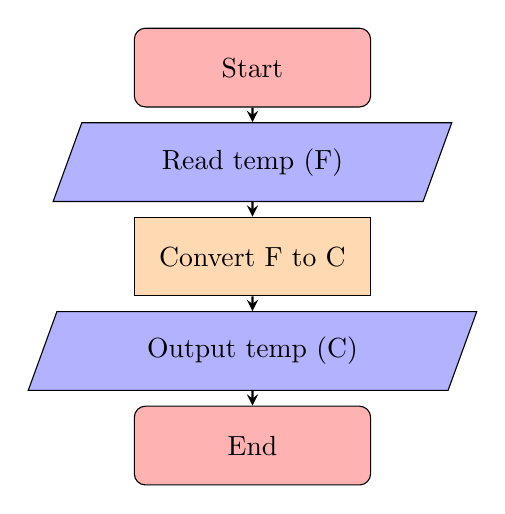
\begin{tikzpicture}[node distance=1.2cm]
      \node (start) [startstop] {Start};
      \node (readF) [io, below of=start] {Read temp (F)};
      \node (convert) [process, below of=readF] {Convert F to C};
      \node (outC) [io, below of=convert] {Output temp (C)};
      \node (end) [startstop, below of=outC] {End};
      \draw [arrow] (start) -- (readF);
      \draw [arrow] (readF) -- (convert);
      \draw [arrow] (convert) -- (outC);
      \draw [arrow] (outC) -- (end);
    \end{tikzpicture}
  \end{figure}
\end{frame}

\begin{frame}{Let's implement}
  \begin{itemize}
    \item Now we know how the program flows, let's put our ideas in code! 
    \begin{itemize}
      \item Input: We don't know how to do
      \item Process: We don't know how to do 
      \item Output: We already know how to do with \texttt{print}
    \end{itemize}
    \item By the way, the action of converting ideas to code is sometimes called \textbf{implementation}
  \end{itemize}
\end{frame}

\section{Reading inputs}
\begin{frame}[fragile]{Reading inputs}
  \begin{itemize}
    \item Inputs in python are read using \texttt{raw\_input} and \texttt{input} function
    \item We shall first try \texttt{input}
    \item According to the \href{https://www.w3schools.com/python/ref_func_input.asp}{documentation},the syntax of \texttt{input} is:
\begin{lstlisting}[language=python]
      input(prompt)
\end{lstlisting}
  where \texttt{prompt} is a string representing a default message before the input.
  \end{itemize}
\end{frame}

\begin{frame}{Reading input}
  \begin{itemize}
    \item What does that even mean?
    \item Let's experiment by opening up the python interactive console
    
  \end{itemize}
  
  \begin{figure}
    \centering
    \includegraphics[width=0.8\textwidth]{img/repl.PNG}
  \end{figure}
\end{frame}

\begin{frame}{Reading input}
  \begin{itemize}
    \item Type in \texttt{input("Enter here:")} and enter
    \item The following should show:
  \end{itemize}
  \begin{figure}
    \centering 
    \includegraphics[width=0.8\textwidth]{img/repl-input-prompt.PNG}
  \end{figure}
\end{frame}

\begin{frame}{Reading input}
  \begin{itemize}
    \item Type something and press enter 
    \item You should see your input displaying:
  \end{itemize}
  \begin{figure}
    \centering 
    \includegraphics[width=0.8\textwidth]{img/repl-input-done.PNG}
  \end{figure}
\end{frame}

\begin{frame}[fragile]{Reading input}
  \begin{itemize}
    \item As you can probably see, \texttt{input} ask you a question which you can answer 
    \item You answer by typing some input and press enter to submit
    \item Furthermore, the text inside \texttt{input} is displayed when it prompts for answer
    \item So you can imagine in our final program the code would have something like this:
    \begin{lstlisting}[language=python]
      input("Enter temperature in (F): ")
\end{lstlisting}
    \item But here is a problem: How can we save and manipulate these input?
  \end{itemize}
\end{frame}

\section{Variables}
\begin{frame}{Why do we need to store?}
  \begin{itemize}
    \item But you may ask, why do we need to save results anyway?
    \item The answer is actually quite obvious: \textit{If you don't remember anything, you can't process anything}
    \item \textit{Example: Guy who forgot everything he heard}
    \item \textit{Imagine asking a forgetful guy what is the difference in age between you and your friends. One by one, you and your friend told the guy your ages. Being forgetful, he never remembers anything he heard. You can see such a guy will never be able to answer your question, because he would have forgotten your age by the time he listen to your friend's!}
  \end{itemize}
\end{frame}
\begin{frame}{Variables - Your handy storage box}
  \begin{itemize}
    \item To store data, a computer uses something called a \textbf{variable}
    \item A variable is a ”storage box” with a name
    \item It stores data temporarily so that the value inside can be retrieved for further processing
  \end{itemize}
  \begin{figure}
    \centering 
    \includegraphics[width=0.6\textwidth]{img/variable.png}
    \caption*{Source: \href{https://stevenpcurtis.medium.com/what-is-a-variable-3447ac1331b9}{https://stevenpcurtis.medium.com/what-is-a-variable-3447ac1331b9}}
  \end{figure}
\end{frame}

\begin{frame}{Three parts of a variable}
  \begin{itemize}
    \item A variable always consist of 3 things:
    \begin{enumerate}
      \item \textbf{Name} for us to refer later in the program 
      \item \textbf{Value} that contain what is stored
      \item \textbf{Data type} that indicate what \textit{kinds} of value is stored
    \end{enumerate}
    \item Name and value is trivial, let's look at data types
  \end{itemize}
\end{frame}

\section{Data types}
\begin{frame}{What is data types?}
  \begin{itemize}
    \item Values in computer are always stored as 0s and 1s 
    \item The same sequence of bits can represent different things according to the way we decode it!
    \item Different data type care stored and manipulate differently by computer!
    \item So important to let the computer knows what \textbf{data types} they are dealing with
  \end{itemize}
\end{frame}

\begin{frame}{Data types: Integer}
  \begin{itemize}
    \item \textbf{Integers} ($\mathbb{Z}$) are \textit{numbers without decimal points and fraction component}
    \item  Examples of integers $\{\cdots, -4, -3, -2, -1 , 0, +1, +2, +3, +4, \cdots\}$
    \item Examples of integral data: \textit{age}, \textit{no. of apples}, \textit{no. of people}
  \end{itemize}
\end{frame}

\begin{frame}{Data types: Float}
  \begin{itemize}
    \item \textbf{Floating point numbers} are \textit{numbers with decimal points}
    \item  Examples of floating point numbers: $2.5$, $0.0$, $-3.1$, $100.173$
    \item Examples of float data: \textit{temperature}, \textit{volume}, \textit{mass}, \textit{height}
  \end{itemize}
\end{frame}

\begin{frame}{Data types: Character}
  \begin{itemize}
    \item \textbf{Character} is \textit{a single character}
    \item Usually quoted by \textbf{single quotes ('')}
    \item Examples of characters numbers: \texttt{'a'},\texttt{'F'},\texttt{'<space>'},\texttt{'@'},\texttt{'0'},\texttt{'+'}
    \item Examples of character data: \textit{grades}
  \end{itemize}
\end{frame}

\begin{frame}{Data types: String}
  \begin{itemize}
    \item \textbf{String} is \textit{a sequence of one or more character}
    \item Usually quoted by \textbf{double quotes ("")}
    \item Examples of string: \texttt{"hello"},\texttt{"ymchan@gmail.com"},\texttt{"1+2=3"},\texttt{"kim\_979"}
    \item Examples of string data: \textit{name}, \textit{email}, \textit{username}, \textit{password}
  \end{itemize}
\end{frame}

\begin{frame}{Data types: Boolean}
  \begin{itemize}
    \item \textbf{Boolean} is a variable either \texttt{true} or \texttt{false}
    \item Usually denote a state, or some flag
    \item Examples of boolean data: \textit{is\_married}, \textit{is\_empty}, \textit{is\_opened}, \textit{is\_running}
  \end{itemize}
\end{frame}


\begin{frame}{Case study I}
  \begin{columns}
    \column{0.6\textwidth}
    \begin{itemize}
      \item Variable name is \textbf{myInt}
      \item The value stored is \textbf{4}
      \item The data are numbers \textit{without decimal points}, so the data type is \textbf{integer}
    \end{itemize}
    \column{0.4\textwidth}
    \begin{figure}
      \includegraphics[width=0.8\textwidth]{img/variable-int.png}
    \end{figure}
  \end{columns}
\end{frame}

\begin{frame}{Case study II}
  \begin{columns}
    \column{0.6\textwidth}
    \begin{itemize}
      \item Variable name is \textbf{myReal}
      \item The value stored is \textbf{2.5}
      \item The data are numbers \textit{with decimal points}, so the data type is \textbf{floating point number}
    \end{itemize}
    \column{0.4\textwidth}
    \begin{figure}
      \includegraphics[width=0.8\textwidth]{img/variable-float.png}
    \end{figure}
  \end{columns}
\end{frame}

\begin{frame}{Case study III}
  \begin{columns}
    \column{0.6\textwidth}
    \begin{itemize}
      \item Variable name is \textbf{myChar}
      \item The value stored is \textbf{"a"}
      \item The data is a \textit{single character}; The data type is \textbf{character}
    \end{itemize}
    \column{0.4\textwidth}
    \begin{figure}
      \includegraphics[width=0.8\textwidth]{img/variable-chr.png}
    \end{figure}
  \end{columns}
\end{frame}

\begin{frame}{Case study IV}
  \begin{columns}
    \column{0.6\textwidth}
    \begin{itemize}
      \item Variable name is \textbf{myString}
      \item The value stored is \textbf{"hello"}
      \item The data is a \textit{sequence of characters}; The data type is \textbf{string}
    \end{itemize}
    \column{0.4\textwidth}
    \begin{figure}
      \includegraphics[width=0.8\textwidth]{img/variable-str.png}
    \end{figure}
  \end{columns}
\end{frame}

\section{Doing things in python}
\subsection{Declaring variables}
\begin{frame}[fragile]{Declaring variables}
  \begin{itemize}
    \item Let's see how all these turn into code:
    \item To \textbf{declare} a variable, do the following
  \begin{lstlisting}[language=python]
    <variable name> = <value>
\end{lstlisting}
    \item For example:
    \begin{lstlisting}[language=python]
      myName = "John" # String variable myName storing "John"

      age = 19 # Integer variable age storing 19
      
      temp = 23.3 # Float variable called temp storing 23.3

      isOk = False # Boolean variable called isOK storing False 
\end{lstlisting}
  \end{itemize}
\end{frame}

\subsection{Accessing values}
\begin{frame}[fragile]{Accessing values}
  \begin{itemize}
    \item After declaration, we can access the values stored by the variable name:
\begin{lstlisting}[language=python]
name = "John"
# This will output "Your name is: John"
print("Your name is:", name) 

temp = 22.1
temp + 1 # 23.1 
temp - 10 # 13.1
# Output: "Temp minus 10: 13.1"
print("Temp minus 10: ", temp - 10) 
\end{lstlisting}
  \end{itemize}
\end{frame}

\subsection{Checking data type}
\begin{frame}[fragile]{Checking data type}
  \begin{itemize}
    \item We can also look at the data type of things using \texttt{type()} function
\begin{lstlisting}[language=python]
  >>> type(1)
  <class 'int'>

  >>> type(1.2)
  <class 'float'>

  >>> type('12')
  <class 'str'>
  
  >>> type(True)
  <class 'bool'>
\end{lstlisting}
  \end{itemize}
\end{frame}

\begin{frame}[fragile]{Checking data type}
  \begin{itemize}
    \item Similarly for variables
\begin{lstlisting}[language=python]
  >>> myName = "John"
  >>> type(myName)
  <class 'str'>

  >>> temp = 30.2
  >>> type(temp)
  <class 'float'>
\end{lstlisting}
  \end{itemize}
\end{frame}

\begin{frame}[fragile]{Checking data type}
  \begin{itemize}
    \item We can also use the \texttt{is} keyword to check if an object belongs to a type 
\begin{lstlisting}[language=python]
>>> age = 20
>>> type(age)
<class 'int'>
>>> type(age) is int
True

>>> myName  = "rs132"
>>> type(myName) is str
True

>>> isDone = False
>>> type(isDone) is bool
True
>>> type(isDone) is int
False
\end{lstlisting}
  \end{itemize}
\end{frame}

\subsection{Doing Operations}
\begin{frame}[fragile]{Doing operations with variables}
  \begin{itemize}
    \item We can also manipulate the values stored in the variable using various operators. For example, if the varaibles are \texttt{int} or \texttt{float}:
\begin{lstlisting}[language=python]
>>> 1.0 + 2.0     # Addition
3.0
>>> 3 - 10        # Subtraction
-7
>>> 3 * 5         # Multiplication
15
>>> 4/3           # Division
1.3333333333333333
>>> 4**5          # Exponent (4**5 = 4*4*4*4*4)
1024
\end{lstlisting}
  \end{itemize}
\end{frame}


\begin{frame}[fragile]{Doing operations with variables}
  \begin{itemize}
    \item Similarly for string, we have the \texttt{+} and \texttt{*} operations defined 
    \item Note that some operations will results in error
\begin{lstlisting}[language=python]
>>> "hello" + "bye"       # Concatenate two string 
'hellobye'
>>> "hello"*3             # Concatenate string 3 times
'hellohellohello' 

>>> "hello" * "bye"       # Make no sense
Traceback (most recent call last):
  File "<stdin>", line 1, in <module>
TypeError: cant multiply sequence by non-int of type 'str'

>>> "hello" - "bye"       # Make no sense 2
Traceback (most recent call last):
  File "<stdin>", line 1, in <module>
TypeError: unsupported operand type(s) for -: 'str' and 'str'
\end{lstlisting}
  \end{itemize}
\end{frame}

\subsection{Saving results}
\begin{frame}[fragile]{Saving results}
  \begin{itemize}
    \item Finally, we can \textbf{assign} our computational results back to string
    \item This is done using the \texttt{=} operator
\begin{lstlisting}[language=python]
>>> i = 5
>>> i + 9       # Won't change i
14
>>> i
5
>>> i = i + 9   # i = xxx Set i to be xxx
>>> i
14
\end{lstlisting}
  \end{itemize}
\end{frame}

\section{Combining everything}

\begin{frame}[fragile]{Combining everything}
  \begin{itemize}
    \item Combining everything, this give us the following code:
\begin{lstlisting}[language=python]
tempF = input("Enter temperature in (F): ")
tempC = 5.0*(tempF - 32.0)/9.0
print("Temperature in (C): ",tempC)
\end{lstlisting}
  \item Let's see how it works out... Ops! An error!
\begin{lstlisting}[language=bash]
>>> python3 temp.py
Enter temperature in (F): 80
Traceback (most recent call last):
  File "temp.py", line 2, in <module>
    tempC = 5.0*(tempF-32.0)/9.0
TypeError: unsupported operand type(s) for -: 'str' and 'float'
\end{lstlisting}
  \end{itemize}
\end{frame}

\begin{frame}[fragile]{What is the error?}
  \begin{itemize}
    \item What is the error? Let's look at the \textbf{error message} more closely:
  \begin{lstlisting}[language=bash]
    File "temp.py", line 2, in <module>
    tempC = 5.0*(tempF-32.0)/9.0
TypeError: unsupported operand type(s) for -: 'str' and 'float'
\end{lstlisting}
  \item According to the message, we are using the subtraction operand (\texttt{-}) to subtract \texttt{str} and \texttt{float}!
  \item But why? Isn't our input \texttt{80} a float?
  \end{itemize}
\end{frame}

\begin{frame}[fragile]{What is the error?}
  \begin{itemize}
    \item  Is it really so? In debugging, it's always good to check our assumptions because sometimes it can be wrong!
    \item Let's check by printing the type of \texttt{tempF}
\begin{lstlisting}[language=python]
tempF = input("Enter temperature in (F): ")
print('Type of tempF: ',type(tempF))
tempC = 5.0*(tempF - 32.0)/9.0
print("Temperature in (C): ",tempC)
\end{lstlisting}
  \end{itemize}
\end{frame}

\begin{frame}[fragile]{What is the error?}
  \begin{itemize}
    \item Let's see what it returns now:
\begin{lstlisting}[language=bash]
>>> python3 temp.py
Enter temperature in (F): 80
Type of tempF:  <class 'str'>    <---- Ops! tempF is a string!!!
Traceback (most recent call last):
  File "temp.py", line 3, in <module>
    tempC = 5.0*(tempF-32.0)/9.0
TypeError: unsupported operand type(s) for -: 'str' and 'float'
\end{lstlisting}
  \end{itemize}
\end{frame}

\begin{frame}[fragile]{What is the error?}
  \begin{itemize}
    \item Turns out, the problem is the way \texttt{input} handles input. According to the \href{https://docs.python.org/3/library/functions.html#input}{documentation}:
  \end{itemize}
  \begin{figure}
    \centering
    \includegraphics[width=0.8\textwidth]{img/python-docs.png}
  \end{figure}
\end{frame}

\begin{frame}[fragile]{What is the error?}
  \begin{itemize}
    \item So basically, \texttt{input} will convert everything we input, regardless of it's original form, into string!
    \item To battle this, we need to \textit{manually} turn \texttt{str} back to \texttt{float}
    \item This is done by wrapping \texttt{float()} in front of \texttt{input}, i.e. from:
\begin{lstlisting}[language=python]
input("Enter temperature in (F): ")
\end{lstlisting}
to
\begin{lstlisting}[language=python]
float(input("Enter temperature in (F): "))
\end{lstlisting}
  \end{itemize}
\end{frame}

\begin{frame}[fragile]{Final code}
  \begin{itemize}
    \item The final code is then:
\begin{lstlisting}[language=python]
tempF = float(input("Enter temperature in (F): ")) 
print('Type of tempF: ',type(tempF))
tempC = 5.0*(tempF - 32.0)/9.0
print("Temperature in (C): ",tempC)
\end{lstlisting}
  \item and finally we can run!
\begin{lstlisting}[language=bash]
>>> python3 temp.py
Enter temperature in (F): 80
Type of tempF:  <class 'float'>
Temperature in (C):  26.666666666666668
\end{lstlisting}
  \end{itemize}
\end{frame}

\begin{frame}[fragile]{Some comment on type casting}
  \begin{itemize}
    \item The trick we used to solve the problem is actually called \textbf{type casting}
    \item Type casting converts data type from one kinds to another
    \item In general, to \textit{cast} a value / variable to \texttt{<data-type>}, do:
\begin{lstlisting}[language=python]
  <data-type>(<value/variable>)
\end{lstlisting}
    \item For example:
\begin{lstlisting}[language=python]
  float("1.2")    # Converts string "1.2" to float 
  int("12")       # Converts string "12" to int 
  str(1.2)        # Converts float 1.2 to string 
\end{lstlisting}
  \end{itemize}
\end{frame}

\section{More exercise}

\subsection{Radius from circumference}
\begin{frame}[fragile]{Radius from circumference}
  \begin{itemize}
    \item Write a program that takes in the circumference of a circle and output the radius of the circle
    \item \textbf{Solution}:
\begin{lstlisting}[language=python]
C  = float(input("Enter circumference")) # Circumference
PI = 3.1415926535 # Pi
r = C/(2*PI)      # Circumference/2 Pi
print("Radius is: ",r)
\end{lstlisting}
  \end{itemize}
\end{frame}

\subsection{Swapping numbers}
\begin{frame}[fragile]{Swapping numbers}
  \begin{itemize}
    \item Complete the following code that swap the values in \texttt{i} and \texttt{j}
\begin{lstlisting}[language=python]
i = 4
j = 6
print("i: ",i, " j: ",j)      # i: 4 j: 6 
# Do something here to swap i,j. Can define new variable
print("i: ",i, " j: ",j)      # i: 6 j: 4
\end{lstlisting}
  \item \textbf{Solution:}
\begin{lstlisting}[language=python]
temp = i
i = j
j = temp
\end{lstlisting}
  \end{itemize}
\end{frame}

\subsection{Length converter}
\begin{frame}[fragile]{Length converter}
  \begin{exampleblock}{Problem}
    We will write something similar to the Fahrenheit to Celsius converter. Instead of converting temperature, we will write code that convert length from miles to kilometer. Write a program that read in length in miles, then output length in kilometer. (Remark: 1 miles $\approx$ 1.60934 km)
  \end{exampleblock}
  \begin{exampleblock}{Expected output}
\begin{lstlisting}
Please enter length in miles: 2.7
Length in kilometer: 4.345218
\end{lstlisting}
  \end{exampleblock}
\end{frame}

\begin{frame}[fragile]{Average Calculator}
  \begin{exampleblock}{Problem}
    Write a program that takes in 5 numbers $x_1,x_2,\cdots,x_5$ and calculate the average of the numbers $\bar{x} = (x_1 + x_2 + x_3 + x_4 + x_5)/5$
  \end{exampleblock}
  \begin{exampleblock}{Expected output}
\begin{lstlisting}
2.5
2.1
4.5
1.2
4.5
Average of these numbers is 2.96
\end{lstlisting}
      \end{exampleblock}
\end{frame}


\subsection{Challenging: Number of hand shakes}
\begin{frame}{Challenging: Number of hand shakes}

  \begin{exampleblock}{Problem}
    $n$ business people meet for lunch and shake hands with each other. How many handshakes are there? (Obviously $n\in \mathbb{Z}^+$)\\
    (Hint: Consider the case when $n=1,2,3,4,5$, can you see a pattern?)
  \end{exampleblock}
\end{frame}

\begin{frame}{Challenging: Number of hand shakes (Answer)}

  \begin{alertblock}{Answer}
    Let $n$ be the number of people and $S_n$ be the number of handshakes.
    \begin{table}[]
      \begin{tabular}{llllllll}
      $n$ & 1 & 2 & 3 & 4 & 5 & 6 & 7\\
      $S_n$ & 0 & 1 & 3 & 6 & 10 & 15 & 21 
      \end{tabular}
      \end{table}
      Observe that $S_n = S_{n-1} + (n-1)$ for $n>1$
  \end{alertblock}
\end{frame}

\begin{frame}{Challenging: Number of handshakes (Answer)}
  Thefore:
  \begin{align*}
    S_n &= S_{n-1} + (n-1) \\
    &= (S_{n-2} + (n-2)) + (n-1)\\
    &= (S_{n-3} + (n-3)) + (n-2) + (n-1)\\
    &= \cdots\\
    &= (S_{2} + 2) + 3 + \cdots + (n-2) + (n-1)\\
    &= (S_{1} + 1) + 2 + 3 + \cdots + (n-2) + (n-1)\\
    &= \mathbf{0 + 1 + 2 + 3 + \cdots + (n-2) + (n-1)}
  \end{align*}
  
\end{frame}

\begin{frame}{Challenging: Number of handshakes (Answer)}
  \begin{equation*}
    S_n = 0 + 1 + 2 + 3 + \cdots + (n-2) + (n-1)
  \end{equation*}
  \begin{itemize}
    \item In fact, it can be shown that $S_n = n(n-1)/2$
    \item This is because each people shakes with $n-1$ people
    \item Since there are $n$ peoples, the number of shakes should be $n(n-1)$
    \item But A shakes B and B shakes A are count the same, so we double counted
    \item Therefore $S_n = n(n-1)/2$
  \end{itemize} 
\end{frame}


\begin{frame}[fragile]{Challenging: Number of handshakes (Answer)}
  Implementation in code:
\begin{lstlisting}[language=python]
n = input('Enter number of people: ')
n = int(n)
Sn = n*(n-1)//2 # // for integer division
print('Total number of handshakes: ', Sn)
\end{lstlisting}
\end{frame}

\end{document}
